%%%%%%%%%%%%%%%%%%%%%%%%%%%%%%%%%%%%%%%%%
% Beamer Presentation
% LaTeX Template
% Version 1.0 (10/11/12)
%
% This template has been downloaded from:
% http://www.LaTeXTemplates.com
%
% License:
% CC BY-NC-SA 3.0 (http://creativecommons.org/licenses/by-nc-sa/3.0/)
%
%%%%%%%%%%%%%%%%%%%%%%%%%%%%%%%%%%%%%%%%%

%----------------------------------------------------------------------------------------
%	PACKAGES AND THEMES
%----------------------------------------------------------------------------------------

\documentclass{beamer}

\mode<presentation> {

% The Beamer class comes with a number of default slide themes
% which change the colors and layouts of slides. Below this is a list
% of all the themes, uncomment each in turn to see what they look like.

%\usetheme{default}
%\usetheme{AnnArbor}
%\usetheme{Antibes}
%\usetheme{Bergen}
%\usetheme{Berkeley}
%\usetheme{Berlin}
%\usetheme{Boadilla}
%\usetheme{CambridgeUS}
%\usetheme{Copenhagen}
%\usetheme{Darmstadt}
%\usetheme{Dresden}
%\usetheme{Frankfurt}
%\usetheme{Goettingen}
%\usetheme{Hannover}
%\usetheme{Ilmenau}
%\usetheme{JuanLesPins}
%\usetheme{Luebeck}
\usetheme{Madrid}
%\usetheme{Malmoe}
%\usetheme{Marburg}
%\usetheme{Montpellier}
%\usetheme{PaloAlto}
%\usetheme{Pittsburgh}
%\usetheme{Rochester}
%\usetheme{Singapore}
%\usetheme{Szeged}
%\usetheme{Warsaw}

% As well as themes, the Beamer class has a number of color themes
% for any slide theme. Uncomment each of these in turn to see how it
% changes the colors of your current slide theme.

%\usecolortheme{albatross}
%\usecolortheme{beaver}
%\usecolortheme{beetle}
%\usecolortheme{crane}
%\usecolortheme{dolphin}
%\usecolortheme{dove}
%\usecolortheme{fly}
%\usecolortheme{lily}
%\usecolortheme{orchid}
%\usecolortheme{rose}
%\usecolortheme{seagull}
%\usecolortheme{seahorse}
%\usecolortheme{whale}
%\usecolortheme{wolverine}

%\setbeamertemplate{footline} % To remove the footer line in all slides uncomment this line
%\setbeamertemplate{footline}[page number] % To replace the footer line in all slides with a simple slide count uncomment this line

%\setbeamertemplate{navigation symbols}{} % To remove the navigation symbols from the bottom of all slides uncomment this line
}
\usepackage[brazil]{babel} % pacote portugues brasileiro
\usepackage[utf8]{inputenc} % pacote para acentuacao direta
\usepackage{graphicx} % Allows including images
\usepackage{booktabs} % Allows the use of \toprule, \midrule and \bottomrule in tables

%----------------------------------------------------------------------------------------
%	TITLE PAGE
%----------------------------------------------------------------------------------------

\title{Proposta de um Modelo para Representar Cenários de Acidentes Usando Conceitos de Normas, Sanções e Violações} % The short title appears at the bottom of every slide, the full title is only on the title page

\author{Jonathan M. Samara \\ Orientador Prof. Dr. Cesar A. Tacla} % Your name
\institute[UTFPR] % Your institution as it will appear on the bottom of every slide, may be shorthand to save space
{
Universidade Tecnológica Federal do Paraná \\ % Your institution for the title page
\medskip
}
\date{\today} % Date, can be changed to a custom date

\begin{document}

\begin{frame}
\titlepage % Print the title page as the first slide
\end{frame}

\begin{frame}
\frametitle{Introdução} % Table of contents slide, comment this block out to remove it
	\begin{itemize}
			\item Muitas pessoas são submetidas a atividades que apresentam algum risco. 
			\item Exemplos de serviços assim; elétrica, petroquímica, telecomunicações, transportes. 
			\item Existe uma série de possíveis causas em um acidente. 
			\item A computação pode contribuir com esse tipo de problema. 
			\item Criar representações para tratar esse problema. 			
	\end{itemize}
\end{frame}

\begin{frame}
\frametitle{Introdução - Motivação} % Table of contents slide, comment this block out to remove it
	\begin{itemize}
			\item Uma maneira de representar cenários assim está relacionado com sistemas multiagentes normativos. 
			\item Dentro deste tipo de atenge é possível observar os conceitos de; norma, violação e sanção.
			\item Portanto, entender como usar agentes normativos para criar representações específicas a problemas envolvendo trabalho, acidente e risco é uma motivação para esse estudo. 
			\item Realizar a análise dos raciocínios que podem ser construído é outra motivação. 			
	\end{itemize}
\end{frame}

\begin{frame}
\frametitle{Introdução - Relevância} % Table of contents slide, comment this block out to remove it
	\begin{itemize}
			\item Contribuição para três campos; Representação Computacional, Sistemas Multiagentes e Segurança.
			\item Representação Computacional e Sistemas Multiagentes.
			\begin{itemize}
				\item Existem modelos para representar Sistemas Multiagentes, porém não apresentar características específicas (conceitos, predicados, regras) para tratar cenários de acidentes. 
				\item Existem modelos para representar SMA Normativos, mas apresentam aspectos altamente genéricos, não tendo características específicas (conceitos, predicados e regras) para tratar cenários de acidentes e riscos.
				\item Existem modelos para representar cenários de acidentes (am ambiente de trabalho) usando \textit{SMA}, contudo são complexos. Além disso, esses modelos não focam no erro dos agentes bem como as consequências dos mesmos sobre os demais colegas.  
			\end{itemize}			 
	\end{itemize}
\end{frame}

\begin{frame}
\frametitle{Introdução - Relevância} % Table of contents slide, comment this block out to remove it
	\begin{itemize}
			\item Segurança
			\begin{itemize}
				\item O interesse da pesquisa é computacional. 
				\item O modelo aqui proposto trata de conceitos relacionados a riscos e situações inesperadas.
				\item Portanto, apesar do interesse ser principalmente computacional, há um diálogo com o campo da Segurança. 
			\end{itemize}			 
	\end{itemize}
\end{frame}

\begin{frame}
\frametitle{Introdução - Objetivo Geral} % Table of contents slide, comment this block out to remove it
	\begin{itemize}
		\item Conceber uma representação que tenha maior expressividade (quando comparado com os demais modelos) ao representar o seguinte cenário; "Agentes trabalham de forma colaborativa para atingir um dado objetivo geral. Esses agentes podem cometer erros submetendo a si mesmos bem como a outros a acidentes ocasionando grandes danos a integridade física do(s) acidentado(s). Não apenas isso, mas essa representação deverá ser capaz de considerar as relações existentes entre as entidades (agentes, artefatos tais como ferramentas), condições ambientais com as violações, sanções e acidentes. Questões envolvendo caráter possibilístico dos acidentes frente a ação dos agentes também deverão ser verificadas nessa representação."  
	\end{itemize}
\end{frame}

\begin{frame}
\frametitle{Introdução - Objetivos Específicos}
	\begin{enumerate}
		\item Representar um SMA. 
		\item Representar normas, violações e sanções sendo que as violações são erros cometidos pelos agentes e as sanções estão relacionadas com os acidentes e suas respectivas consequências.
		\item Representar situações onde um agente é submetido a um evento ruim (integridade física do agente é negativamente afetada de alguma maneira) mesmo que ele não tenha cometido erro algum. 
		\item Representar como se dá as relações entre as entidades, condições ambientes e conjunto coma s violações e sanções. 
		\item Representar as possibilidades da ocorrência de um evento atrelado a um dado risco. 
	\end{enumerate}
\end{frame}


\begin{frame}
\frametitle{Fundamentação Teórica - Agentes}
	\begin{itemize}
		\item Um agente é um sistema computacional que está situado em um dado ambiente e que apresenta comportamento autônomo com a finalidade de atingir um dado objetivo que a ele é designado. 
		\item Ambiente
		\begin{itemize}
			\item Acessibilidade vs Inacessibilidade; Quanto mais acessível for o ambiente mais o agente consegue ter informações claras, precisas e atualizadas. 
			\item Determinístico vs Não-Determinístico; Quanto mais determinístico for o ambiente mais uma ação possui um comportamento claro e determinístico sem incertezas do estado resultante. 
			\item Episódico vs Não-Episódico; Um ambiente tende a ser o mais episódico possível tanto
			quando o desempenho do agente estiver associado a um episódio discreto e específico no
			ambiente.			
			\item Estático vs Dinâmico; Um ambiente é estático se não houver outros processos em paralelo aos eventos associados ao agente.
			\item Discreto vs Contínuo; Um ambiente é discreto se existe um número finito de ações e percepções. 
		\end{itemize}
	\end{itemize}
\end{frame}

\begin{frame}
\frametitle{Fundamentação Teórica - Agentes}
	\begin{itemize}
		\item Uma entidade autônoma é uma entidade que apresenta a capacidade de agir por si mesma. 
		\item Um termostato é uma entidade autônoma. 
		\item Programas de Servidor Daemon são exemplos de entidades autônomas. 
		\item Esses exemplos são apropriados para serem retratados por agentes, contudo não são bons exemplos de agentes inteligentes. 
		\item Um agente inteligente deve apresentar as definições já tratadas e mais as seguintes propriedades; reatividade, proatividade e habilidades sociais.  
		\item Existe duas categorias de Agentes; puramente reativos (tomam decisões considerando apenas o instante presente).
		\item Existe duas categorias de Agentes; possuem estado; possuem uma dada estrutura de dados interna que são considerados quando o agente toma uma certa decisão.
	\end{itemize}
\end{frame}

\begin{frame}
\frametitle{Fundamentação Teórica - Agentes}
	\begin{itemize}
		\item Arquitetura de Agentes Inteligentes;
		\begin{itemize}
			\item Agentes baseados em Lógica; realizam deduções para efetuar uma dada decisão.
			\item Agentes reativos; realizam o mapeamento de uma situação sobre uma ação. 
			\item Agentes BDI; apresenta estados de crenças, desejo e intenções.
			\item Agentes em camadas; tomada de decisão acontece por meio de uma estrutura em camadas que gera um nível de abstração extremamente elevando sobre questões do ambiente. 
		\end{itemize}
	\end{itemize}
\end{frame}

\begin{frame}
\frametitle{Fundamentação Teórica - Artefatos}
	\begin{itemize}
		\item Um agente pode ser estruturado em termos \textit{goal-governed} e \textit{goal-oriented}.
		\item Os agentes \textit{goal-governed} têm capacidades cognitivas e podem representar os seus respectivos objetivos. 
		\item Os agentes \textit{goal-oriented} são programados para alcançar um dado objetivo. 
		\item Artefatos não se enquadram nessas duas características. Essas entidades são exploradas pelo agente para que eles possam alcançar um dado objetivo. 
		\item Em termos mais formais, artefato apresenta as seguintes propriedades; interfaces de uso, instruções de operação, funcionalidade e estrutura de comportamento. 
	\end{itemize}
\end{frame}

\begin{frame}
\frametitle{Fundamentação Teórica - Artefatos}
	\begin{itemize}
		\item Interface de uso são as operações que podem ser invocadas pelos agentes. 
		\item Instruções de operação consiste nas descrições de como fazer uso dessas operações.
		\item Funcionalidade consiste no propósito definido pelo programador. 
		\item Estrutura de Comportamento; consiste nos aspectos internos do artefato a fim de providenciar as funcionalidades. 
	\end{itemize}
\end{frame}

\begin{frame}
\frametitle{Fundamentação Teórica - Artefatos}
	\begin{itemize}
		\item Cartago é um \textit{framework} usado para especificar as relações entre agentes e artefatos e é composto por três blocos; \textit{agent bodies, artefact} e \textit{workspace}. 
		\item \textit{Agent Bodies}; Possibilita a inteligência do agente se relacionar com o meio.
		\item \textit{Artifacts}; São os tijolos lógicos do Cartago. Cada \textit{Artifact} contem um id único, um nome lógico (para o agente poder se referenciar) e um nome completo que inclui o nome dos \textit{workspaces} onde estão logicamente contidos. 
		\item A localização lógica dos artefatos se dá em um \textit{workspace} e tem como finalidade definir uma topologia do ambiente de trabalho.   
	\end{itemize}
\end{frame}

\begin{frame}
\frametitle{Fundamentação Teórica - SMA}
	\begin{itemize}
		\item Um sistema multiagente é constituído por agentes autônomos que interagem visando um propósito em comum tendo como consequência um comportamento global. 
		\item Uma organização com essas características, portanto, apresenta em comum; cultura, memória, história, distribuição de atividades e capacidade de distinguir um agente em específico. 
		\item Uma organização de sistema multiagente deve conter relações sociais no que tange a agentes, institutos específicos e grupos sociais. 
		\item Por ser uma organização, uma \textit{SMA} apresenta; Divisão de tipos de atividades, integração, composição, estabilidade/flexibilidade, coordenação, recursividade, representação multinível e causalidade, potenciais e diferenciais, regras e gramáticas.
	\end{itemize}
\end{frame}

\begin{frame}
\frametitle{Fundamentação Teórica - SMA}
	\begin{itemize}
		\item MOISE+ é um formalismo de SMA. Analisar o MOISE+ permite compreender uma \textit{SMA}. 
		\item MOISE+ define três tipos de especificação; estrutural, funcional e deôntica. 
		\item A especificação estrutural;
	\begin{eqnarray}
			\rho_a \sqsubset \rho_b
		\end{eqnarray}
		\begin{eqnarray}\nonumber
			link(\rho_s,\rho_d,auth) \to link(\rho_s,\rho_d,com) \nonumber \\
			link(\rho_s,\rho_d,com) \to link(\rho_s,\rho_d,acq) 
		\end{eqnarray}
		\begin{eqnarray}\nonumber
			link(\rho_s,\rho_d,t) \wedge \rho_s' \sqsubset \rho_s' \to link(\rho_s',\rho_d,t) \nonumber \\
			link(\rho_s,\rho_d,t) \wedge \rho_d' \sqsubset \rho_d' \to link(\rho_s,\rho_d',t) 	
		\end{eqnarray}
		\begin{equation}
			\rho_a \bowtie \rho_b \wedge \rho_a \neq \rho_b \wedge \rho_a \sqsubset \rho' \to \rho' \bowtie \rho_b 
		\end{equation}
		\begin{equation}
			gt = \langle R,SG,L^{intra},L^{inter},C^{intra},C^{inter},np,ng\rangle 
		\end{equation}		 
		\end{itemize}
	\end{frame}
\begin{frame}
\frametitle{Fundamentação Teórica - SMA}
	\begin{itemize}
		\item Especificação funcional; 
	\end{itemize}
	\begin{figure}[H]
	  \centering
	  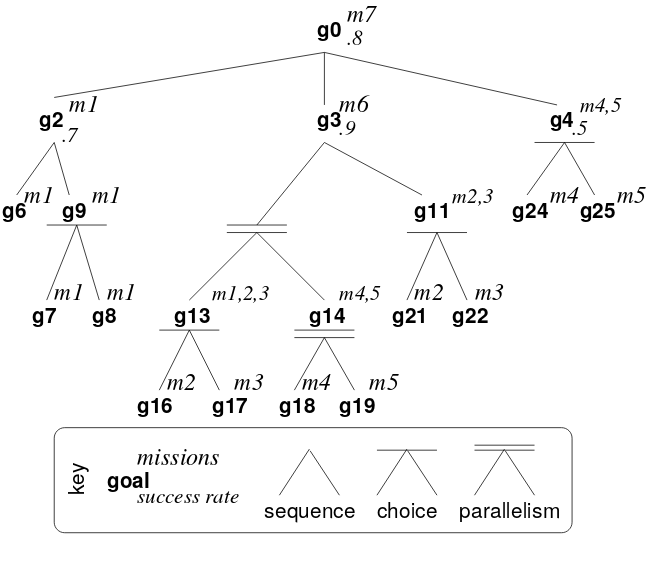
\includegraphics[width=0.4\linewidth]{figure/figmoise} 
	  \caption{Arvore de objetivos definido pelo modelo MOISE+}
	  \label{arvoremoise}
	\end{figure}
	\begin{eqnarray}
		m_k = \{ g_n,...,g_m\}
	\end{eqnarray}

\end{frame}
\begin{frame}
\frametitle{Fundamentação Teórica - SMA}
	\begin{itemize}
		\item Especificação Deôntica; 
	\end{itemize}
	\begin{eqnarray}\nonumber
		obl(\rho,m,tc) \to per(\rho,m,tc) \\
		obl(\rho,m,tc) \wedge \rho \sqsubset \rho' \to obl(\rho',m,tc) \\
		per(\rho,m,tc) \wedge \rho \sqsubset \rho' \to per(\rho',m,tc) \\	
	\end{eqnarray}
\end{frame}

\begin{frame}
\frametitle{Fundamentação Teórica - Normas}
	\begin{itemize}
		\item Há estudos que tratam normas com objetivo de representar sociedades, organizações e instituições.
		\item Há estudos que tratam normas como forma dos agentes trabalharem de maneira coordenada a fim de atingir um dado objetivo. 
		\item No MOISE+ normas são tratadas sobre a ótica da lógica deôntica e é usada para especificar missões aos papeis dos agentes.
		\item Contudo nesse estudo as normas são tratadas tendo como base o modelo do DASTANI. 
	\end{itemize}
\end{frame}

\begin{frame}
	\frametitle{Fundamentação Teórica - Normas}
	\begin{figure}[H]
	  \centering
	  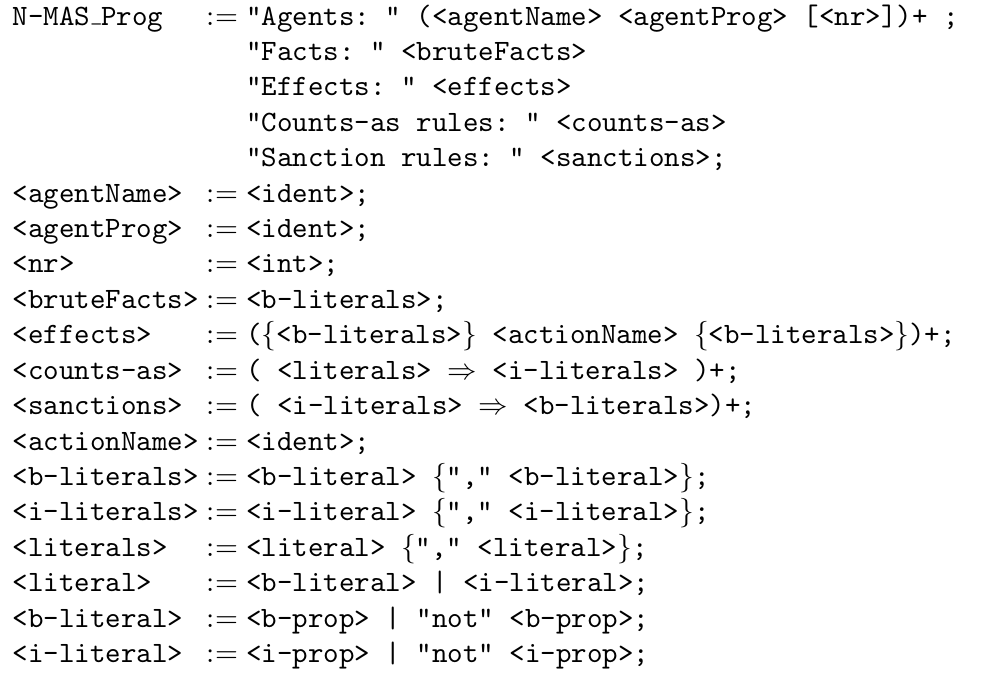
\includegraphics[width=0.5\linewidth]{figure/masprogram.png} 
	  \caption{Linguagem para descrever um programa de multiagentes normativos com a possibilidade de violações e sanções na notação EBNF segundo o texto \cite{dastaniframework}. Nesta notação, $<ident>$ é usado para denotar uma \textit{string} e $<int>$ inteiros. Os termos $<b-prop>$ e $<i-prop>$ são usados para designar dois tipos de conjuntos de proposições que são disjuntos entre si}
	  \label{descreveprograma}
	\end{figure}
\end{frame}

\begin{frame}
	\frametitle{Fundamentação Teórica - Riscos}
	\begin{itemize}
		\item Os erros em industria não podem ser definidos apenas nas falhas de humano. 
		\item Consequência de um comportamento global da instituição contribuem para os erros. 
		\item Esse comportamento advêm de uma forte pressão tendo em vista eficiência e otimização dos processos de produção. 
	\end{itemize}
\end{frame}

\begin{frame}
	\frametitle{Fundamentação Teórica - Riscos}
	\begin{itemize}
		\item BATU - \textit{Boundary Activities Tolerated during Use} (Atividades Limites Toleradas Durante o Uso). Muitas vezes a equipe adota atividades paliativas a fim de otimizar os processos de produção. Isso envolve assumir níveis de tolerância no que diz respeito ao desempenho e a segurança. 
		\item BCTU - \textit{Boundary Conditions Tolerated by Use} (Condições Limites Toleradas Durante o Uso). O termo condição faz referência a uma situação, um estado, circunstâncias externas às quais pessoas ou até mesmo entidades são afetados no que diz respeito a uma certa decisão atrelada a circunstâncias ambientais, materiais, humanas, de produtos e entre outras.
	\end{itemize}
\end{frame}

\begin{frame}
	\frametitle{Metodologia - Levantamento de Requisitos}
	\begin{itemize}
		\item Os requisitos são derivados de uma análise dos Objetivos Específicos desse estudo.
		\item Apresentam as seguintes características; 
		\begin{itemize}
			\item São estáticos (uma vez formulado o problema, não mudam com o decorrer do desenvolvimento da representação);
			\item São articulados em um vocabulário compreensível para os pesquisadores			
		\end{itemize}
	\end{itemize}
\end{frame}

\begin{frame}
	\frametitle{Metodologia - Conceitualização}
	\begin{itemize}
		\item Investigação de modelos que podem ser aplicados a essa situação.
		\item Verificação dos conceitos em interesse dentro desses modelos. 
		\item Os pesquisadores isolaram os conceitos e suas relações nesses modelos. 
		\item Os conceitos ão adaptados ao cenário que se deseja representar.
		\item A estrutura resultante é escrita no seguinte formalismo; Teoria de Conjuntos para representar os conceitos e lógica de predicados para representar as relações. 
		\item UML também é usado para essa mesmo propósito. 
		\item Uma vez feito isso, os pesquisadores constroem regras para determinar a transição as transições de estado.
	\end{itemize} 
\end{frame}

\begin{frame}
	\frametitle{Metodologia - Análise do Estudo de Caso}
	\begin{itemize}
		\item Manutenção em Linha Viva. 
		\item Estudo de manuais técnicos. 
		\item Entrevista com o Engenheiro de Manutenção de Linha Viva. 
		\item Acompanhamento de um procedimento de Manutenção. 
	\end{itemize} 
\end{frame}

\begin{frame}
	\frametitle{Metodologia - Especificação do Estudo de Caso}
	\begin{itemize}
		\item O cenário a ser retratado é; Método a Distância para troca de um isolador de Pedestal. 
		\item É feito um Modelo Baseado em Cenários que consiste na descrição da atividade em linguagem natural. Esse modelo foi verificado por profissionais da área. 
		\item Desse houve o processo de especificação nos conjuntos e predicados definidos anteriormente. 
	\end{itemize} 
\end{frame}

\begin{frame}
	\frametitle{Metodologia - Validação}
	\begin{itemize}
		\item Uma vez com a manutenção especificada, os pesquisadores geraram raciocínios para traduzir diferentes cenários de trabalho (com o propósito de provar a hipótese desse estudo). 
		\item A validação desses raciocínios se dá em análise com o modelo de cenários, pois isso permite verificar se esses raciocínios correspondem com a realidade. 
	\end{itemize} 
\end{frame}

\begin{frame}
	\frametitle{Resultados}
	\begin{figure}[H]
	  \centering
	  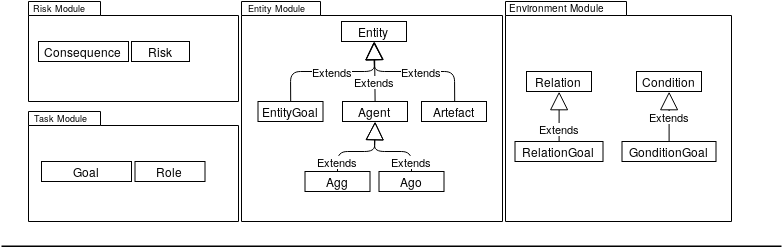
\includegraphics[width=1\linewidth]{figure/Module.png} 
	  \caption{A estrutura geral das classes do modelo}
	  \label{module}
	\end{figure} 
\end{frame}

\begin{frame}
	\frametitle{Resultados - Estrutural Conceitual - Módulos}
 	\begin{equation} 
		M_{Entity} = \{ Entity, Agent, Artefact, EntityGoal, Agg, Ago\}
	\end{equation}\label{modent}

	\begin{equation} \label{defineentity} 
		( Agent \cup Artefact ) \subset Entity
	\end{equation}

	\begin{equation} \label{agentsartefactvoid}
    	Agent \cap Artefact = \emptyset
	\end{equation}

	\begin{equation}
    	M_{Task} = \{ Goal, GoalPreRequisite, Role \}
	\end{equation}

	\begin{equation}
	    M_{Environment} = \{ Relation, ReationGoal, Condition, ConditionGoal \}
	\end{equation}

\end{frame}

\begin{frame}
	\frametitle{Resultados - Estrutural Conceitual - Predicados}
	\begin{equation}
		thereIsRelation(r_l,e_i,e_k) | r_l \in Relation \wedge  e_i, e_k \in Entity
	\end{equation}
	\begin{equation}	
		hasRole(ag_n,\rho_m) | ag_n \in Agent \wedge \rho_m \in Role 	
	\end{equation}
	\begin{equation}	
		hasObligation(\rho_m,g_j) | \rho_m \in Role, g_j \in Goal 
	\end{equation}		
	\begin{equation}	
		hasPermission(\rho_m, g_j) | \rho_m \in Role, g_j \in Goal
	\end{equation}
	\begin{equation}		
		isReached(g_k) | g_k \in Goal 
	\end{equation}
	\begin{equation}			
		stopIn(g_n, ag_m) | g_n \in Goal, ag_m \in Agent
	\end{equation}
	\begin{equation}			
		nextGoal(g_i,g_j) |g_i, g_j \in Goal
	\end{equation}
	\begin{equation}				
		hasCondition(g_i,cg_n) | g_i \in Goal, cg_n \subset GoalCondition
	\end{equation}
	\begin{equation}				
		hasEntity(g_i,eg_m) | g_i \in Goal, eg_m \subset EntityGoal 
	\end{equation}

\end{frame}

\end{document} 	